\documentclass[12pt, dvipsnames]{beamer}
\usepackage{multicol} %multicolumns
\usepackage{siunitx} %log table stuff
\usepackage{flafter}
\usepackage{amsmath} %math stuff
\usepackage{amssymb} %math symbols
\usepackage{graphicx} %including photos
\usepackage{wrapfig} %for wrapping figure
%\graphicspath{{./Report For Titanium Doping/}} %path of folder from where photo needs to be extracted, NOT NECESSARY AT ALL TIMES
\usepackage[utf8]{inputenc}
\usepackage{float} %Using [H] command to stop picturefloating around
\usepackage{enumerate} %changing labels of lists
\usepackage{fancyhdr}
\usepackage{dsfont} %for set notations and other fancy letters
\usepackage{mathrsfs}
\usepackage[compat=1.1.0]{tikz-feynman}

%\usepackage{geometry}
%\geometry{
%a4paper,
%total={170mm,257mm},
%top=20mm,
%}
\usepackage{array}
\setlength\extrarowheight{4pt}
%\usepackage[dvipsnames]{xcolor} %for using coloured text
\usepackage{longtable,pdflscape,booktabs} % long table stuff
\usepackage{lscape} 
\usepackage{caption}
\captionsetup{labelformat=empty}
\usepackage{setspace} %for desired spacing between lines
\usepackage{blindtext} % for blind text in contents page
\usepackage[normalem]{ulem} %dash and dotted underline
\usepackage{bm} % for bold math symbols- using command \boldsymbol
\usepackage{mathtools} %for rcases
\usepackage{hyperref} %for hyperlinks
\usepackage{romannum} %for Roman Numerals
\usepackage[makeroom]{cancel} % for striked out or other stuff in math environment
\usepackage{tikz}
\usepackage{empheq} %  fancy math stuff
\usepackage{xfrac}
\usepackage{fancybox} %for fancy boxes


\allowdisplaybreaks
\colorlet{linkequation}{blue} %making coloured equation refernces

\usetikzlibrary{shadows} %defines shadows
\usepackage[framemethod=tikz]{mdframed}
\usepackage{tcolorbox} %coloured boxes

\tikzset{rndblock/.style={rounded corners,rectangle,draw,outer sep=1pt,inner sep=5pt,line width=1pt}}

% Command Definition
% 1 optional to customize the aspect, 2 mandatory: text to be framed
\newcommand{\mybox}[2][]{\tikz[baseline=(h.base)]\node[rndblock,#1] (h) {#2};}

%definining new command to make coloured equation references
\newcommand*{\myref}[1]{%
  \begingroup
    \hypersetup{
      linkcolor=linkequation,
      linkbordercolor=linkequation,
    }%
    \ref{#1}%
  \endgroup
}

%Setting equations a particular colour
\hypersetup{
colorlinks=true,
linkcolor=black,
filecolor=magenta,
urlcolor=Black,
citecolor=blue,
}

\parskip 1ex

%For circled numbers
\newcommand*\circled[1]{\tikz[baseline=(char.base)]{
            \node[shape=circle,draw,inner sep=2pt] (char) {#1};}}
            
%command for making capital roman numerals
%\newcommand{\RomanNum}[1]{\MakeUppercase{\romannumeral #1}}

%%%%%%%%%%% FOR PRESENTATIONS %%%%%%%%%%%%%%%%%%%%%%%%%%%
\usepackage{beamerthemesplit}
\usetheme{Warsaw}
\usecolortheme{orchid}
\setbeamertemplate{headline}{}
\setbeamercolor*{section in sidebar}{bg=white}
\setbeamercolor*{subsection in sidebar}{fg=black,bg=pink}

\AtBeginSection[]{    
    \begin{frame}{Outline}
    \footnotesize{\tableofcontents[currentsection,hideothersubsections]}
    \end{frame}
}

\begin{document}
%title page
\begin{frame}
    \vspace{\fill}
    \begin{beamercolorbox}[sep=8pt, center,shadow=true, rounded=true]{title}
        \usebeamerfont{subtitle}
        Presentation on \linebreak
        \usebeamerfont{title}
        Antenna Simulation for 21cm H line
    \end{beamercolorbox}
    \begin{center}
      \footnotesize{
        Ashmita Panda \linebreak
        1811042 \linebreak
        4th Year Integrated M.Sc.\linebreak
        SPS, NISER \linebreak

        November 25, 2021 \linebreak
      }
    \end{center}
\end{frame}

%
% section - 21cm Hydrogen line
\section{21cm Hydrogen Line}
%subsection - What is the 21cm Line
\subsection{What is the 21cm Hydrogen Line?}
\begin{frame}{What is the 21cm Hydrogen Line?}
    \begin{itemize}
        \item Neutral hydrogen is made up of an electron and a proton.
        \item The electron and proton both have half-integer spins. 
        \item Neutral hydrogen can exist in two energy states, one with electron and proton spins parallel, and one with antiparallel.
        \begin{figure}
            \centering
            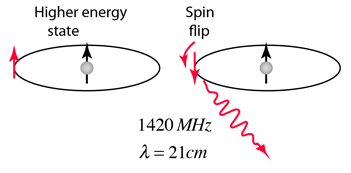
\includegraphics[width=0.6\textwidth]{Images/hflip.png}
            \caption{\tiny Source : \url{http://hyperphysics.phy-astr.gsu.edu/hbase/quantum/h21.html}}
        \end{figure}
    \end{itemize}
\end{frame}
%subsection - Importance in Astrophysics and Cosmology
\subsection{Importance of the 21cm line}
\begin{frame}{Importance of the 21cm line}
    \begin{itemize} 
        \item \uline{In Radio Astronomy} : The rotation curve of galaxy can be measured by observing the 21cm line received from each line of sight.
        \item \uline{In Cosmology} : The ``dark ages'' of the Universe can be probed by using 21cm line.
        \begin{figure}
            \centering
            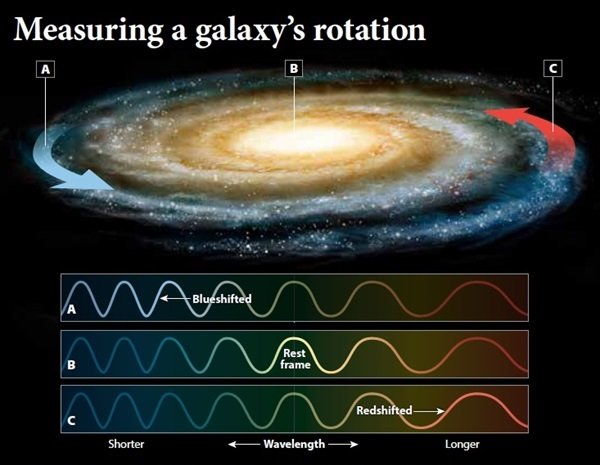
\includegraphics[width=0.5\textwidth]{Images/GalaxyRotation.jpg}
            \caption{\tiny Source : \url{https://physicsopenlab.org/2020/09/08/measurement-of-the-milky-way-rotation/}}
        \end{figure}
    \end{itemize}
\end{frame}

% 
%section - Waveguide
\section{Waveguides}
%subsection - What are Waveguides?
\subsection{What are Waveguides?}
\begin{frame}{What are Waveguides?}
    \begin{itemize}
        \item A waveguide is a structure which guides waves (like EM and sound waves) in a particular direction with minimal energy loss.
        \item A hollow metallic tube is used for guiding EM waves.
        \begin{figure}
            \centering
            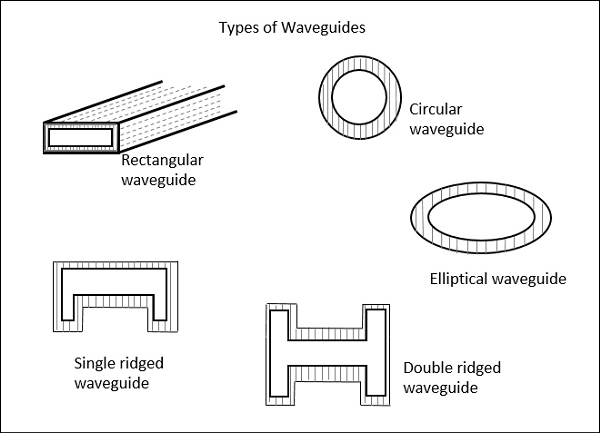
\includegraphics[width=0.6\textwidth]{Images/types_of_waveguides.jpg}
            \caption{\tiny Source : \url{https://www.tutorialspoint.com/microwave_engineering/microwave_engineering_waveguides.htm}}
        \end{figure}
    \end{itemize}
\end{frame}
%subsection - Rectangular Waveguides
\subsection{Rectangular Waveguides}
\begin{frame}{Rectangular Waveguides}
    \begin{itemize}
        \item Rectangular waveguide is one type of waveguide.
        \item The EM waves will be travelling along the z-direction.
        \item Thus, the EM wave solutions for Maxwell equations can be separated into longitudinal and transverse waves.
        \begin{align*}
            E(x,y,z)&=E(x,y)\exp(-i\beta z) \\
            B(x,y,z)&=B(x,y)\exp(-i\beta z)
        \end{align*}
        \begin{figure}
            \centering
            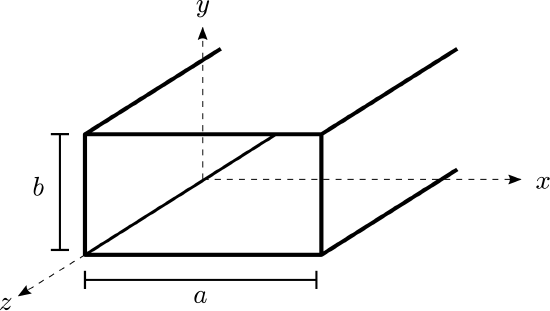
\includegraphics[width=0.5\textwidth]{Images/rectangular.png}
            \caption{\tiny{Source : \url{https://www.tutorialspoint.com/microwave_engineering/microwave_engineering_waveguides.htm}}}
        \end{figure}
    \end{itemize}
\end{frame}


\end{document}